% besdoc.tex V1.0, 17 March 2011

\documentclass[times,mee,doublespace,]{besauth2}
%%\documentclass[times,mee,]{besauth}

\newcommand{\journalnamelc}{British Ecological Society}
\newcommand{\journalabb}{British Ecological Society}
\newcommand{\journalclassshort}{BES}
%%\newcommand{\journalname}{British Ecological Society}
\usepackage{epstopdf}

\usepackage{moreverb}

\usepackage[colorlinks,bookmarksopen,bookmarksnumbered,citecolor=red,urlcolor=red]{hyperref}


\usepackage{lineno}

\newcommand\BibTeX{{\rmfamily B\kern-.05em \textsc{i\kern-.025em b}\kern-.08em
T\kern-.1667em\lower.7ex\hbox{E}\kern-.125emX}}

\bibpunct[; ]{(}{)}{;}{}{}{,}

\def\volumeyear{2015}
\def\VOC{VO}

\begin{document}
\runningheads{P.~B.~Conn, D.~S.~Johnson, \& J.~T.~Thorson}{Preferential sampling in species distribution models}

\papertype{Article}

\title{Confronting preferential sampling in count and occupancy surveys: diagnosis and triage \footnotemark[2]}

\author{Paul B. Conn\affil{1}\corrauth, Devin S. Johnson\affil{1}, James T. Thorson\affil{2}}


\address{\affilnum{1}National Marine Mammal Laboratory, Alaska Fisheries Science Center, NOAA National Marine Fisheries Service, 7600 Sand Point Way NE, Seattle, WA 98115 USA; \affilnum{2} Fisheries Resource Assessment and Monitoring Division (FRAM), Northwest Fisheries Science Center, National Marine Fisheries Service (NMFS),
NOAA, 2725 Montlake Boulevard E, Seattle, WA 98112, USA}

\corraddr{paul.conn@noaa.gov}

\begin{abstract}
 %\noindent {\emph{Summary}}
\small
\begin{enumerate}
\item  Count and occupancy surveys are often used to estimate the density, abundance, and distribution of animal populations. Recently, model-based approaches to analyzing survey data (i.e. species distribution models) have become popular because one can more readily accommodate departures from pre-planned survey routes and construct more detailed maps than one can with design-based procedures. Model-based analysis often makes use of species-covariate relationships and/or spatially autocorrelated random effects to help predict density or occurrence in unsampled locations.

\item Species distribution models often make the implicit assumption that locations chosen for sampling and animal abundance are conditionally independent given modeled covariates.  However, this assumption is likely violated in many cases when survey effort is non-randomized, leading to preferential sampling.

\item We develop a hierarchical statistical modeling framework for detecting and alleviating the biasing effects of preferential sampling in species distribution models.  The approach works by jointly modeling animal abundance/occurrence and the locations selected for sampling, and specifying a dependent correlation structure between the two models.

\item Using simulation, we show that our approach reduces bias resulting from non-random, preferential sampling relative to a traditional species distribution model.  Under strong preferential sampling, biases using traditional species distributions models can be considerable (e.g. 20\%).

\item Species case study

\item When animal populations are surveyed using a non-randomized design, we argue that ecologists routinely test and correct for preferential sampling when fitting species distribution models to animal encounter data.

\end{enumerate}


 Word count: XXXX
\end{abstract}

\keywords{count data, preferential sampling, spatial autocorrelation, species distribution model}

\maketitle \linenumbers

\def\VAR{{\rm Var}\,}
\def\COV{{\rm Cov}\,}
\def\Prob{{\rm P}\,}



\section{Introduction}

Surveys of unmarked animal populations are often used to estimate abundance and occurrence of animal populations and to predict species distributions, enterprises central to conservation, ecology, and management. For studies of abundance, researchers historically relied on design-based statistical inference \citep[e.g.][]{Cochran1977}, which requires adoption of a pre-defined sampling frame (e.g. using systematic random sampling, stratified random sampling, or some variant thereof).  Designing animal surveys is relatively straightforward in such applications, and unbiased point and variance estimators are available.  Recently, however, there has been a surge in research describing model-based procedures for estimating abundance, density, and occupancy from surveys of unmarked animals, including N-mixture models for repeated point counts \citep{Royle2004a}, occupancy models for presence-absence surveys \citep{MacKenzie2002,JohnsonEtAl2013}, and various model-based formulations for distance-sampling data \citep{HedleyBuckland2004,MillerEtAl2013,JohnsonEtAl2010}.  In such applications, it is common to use habitat or environmental covariates together with spatial effects (e.g. via trend surfaces or spatial random effects) to predict density or distributions across the landscape.  We shall refer to the amalgam of model-based approaches for making spatially explicit inference about animal populations as ``Species distribution models" \citep[SDMs; {\it sensu}][]{ElithLeathwick2009}, even though this term is more often used to refer to animal occurrence than it is to density or abundance.

One of the main advantages of using SDMs advanced in the literature is that one is no longer beholden to predetermined sampling frames, and can potentially use data gathered from non-randomized designs or platforms of opportunity to make inferences about animal populations \citep{JohnsonEtAl2010}.  However,
in a recent paper, \citet{DiggleEtAl2010} emphasized that spatially explicit statistical models can easily provide biased estimates when sampling is nonrandom. The potential for biased estimates arises when sampling locations disproportionately target locations where the response of interest is higher (or lower) than the mean response than would be predicted from explanatory covariates with complete knowledge of the system.  In the context of SDMs, this might occur if sampling disproportionately occurs in locations where animals are known to be present or of high abundance, regardless of predictive covariates. For example, if volunteer inventory participants have access to multiple sites with similar covariate values, bias might arise if they consistently choose sites where species are thought or known to be present.  Bias might also arise if surveying effort is higher near bases of operations, and if animal abundance is higher (or lower) near bases of operations than elsewhere in the landscape.


In this article, we explore potential for bias in SDMs resulting from preferential sampling (hereafter, PS), and describe several model-based approaches for detecting and correcting for such biases.  We start by describing a common currency for notation and basic model structures considered in this paper.  Second, we review preferential sampling bias in a mathematical light, and describe prior approaches to coping with its effects. Third, we introduce a novel generalization of previously proposed PS models, allowing the investigator to jointly model animal encounter data and the locations chosen for sampling, including possible dependence structure between these two types of observations.  Fourth, we conduct a simulation study to examine the performance of traditional SDMs and our newly developed PS model when data are gathered preferentially.  Finally, we demonstrate utility of our proposed modeling approach by analyzing a data set of MYSTERY SPECIES X.


\section{Materials and methods}


\subsection{Notation and basic model structures}

We focus here exclusively on discrete space (areal) models for animal encounter data as these seem to be the dominant form used in design and analysis of animal population surveys, although we note that preferential sampling is likely to affect analyses similarly regardless of the choice of spatial domain.  We suppose that the investigator intending to fit a SDM to animal encounter data breaks their study area up into $S$ survey units (label these $U_1, U_2, \hdots, U_S$), of which $n$ are selected for sampling (call the set of sampled locations $\mathcal{S}$). Each survey unit $i$ is assigned a vector of covariates, ${\bf x}_i$, and an indicator $R_i$ that takes on the value 1.0 if survey unit $i$ is sampled (i.e. if $U_i \in \mathcal{S}$), and is 0 otherwise.  To formulate a ``traditional" SDM, one could then write animal abundance or occurrence as a stochastic realization of a probability mass function $f()$:
\begin{eqnarray}
  \label{eq:process}
  Z_i & \sim & f(g^{-1}(\mu_i)).
\end{eqnarray}
In this example, $Z_i$ denotes the state variable of interest (e.g., occupancy or abundance), $g()$ is a link function (e.g. probit or logit for occupancy, log for count data), and $\mu_i$ is a linear predictor.  In applications described in this paper, we write the linear predictor as
\begin{eqnarray}
\mu_i & = & \beta_0 + {\bf x}_i \boldsymbol{\beta}+\eta_i+\epsilon_i,
 \label{eq:mu}
\end{eqnarray}
where $\beta_0$ is an intercept parameter, ${\bf x}_i$ is a row vector of $m$ predictive covariates associated with site $i$, $\boldsymbol{\beta} = \{ \beta_1, \beta_2, \hdots, \beta_m \}$ is a column vector of $m$ regression parameters, $\eta_i$ is a spatially autocorrelated random effect, and $\epsilon_i$ is Gaussian error.  For occupancy, $f()$ would typically be Bernoulli, while the Poisson or negative binomial are typically choices for analysis of count data; common forms for $\eta_i$ include geostatistical specifications \citep{Cressie1993,DiggleEtAl1998}, Gaussian Markov random fields \citep[e.g. conditionally autoregressive models;][]{RueHeld2005}, or low rank alternatives such as predictive process \citep{BanerjeeEtAl2008,LatimerEtAl2009} or restricted spatial regression models \citep{Reich2006,Hughes2013}.

The model for $Z_i$ describes variation in the process of interest and is often described as the ``process'' model.  However, it is usually impossible to observe the system perfectly even in locations where sampling occurs, so it is customary to include an observation model describing incomplete detection.  For occupancy studies, the response variable $Y_i = 1$ if the species of interest is detected and is 0 otherwise, and is modeled with a Bernoulli distribution \citep{Royle2008}
\begin{eqnarray}
  Y_i & \sim & \text{Bernoulli}(Z_i p_i),
\end{eqnarray}
where $p_i$ is possibly a function of survey and observer specific covariates. Replicate surveys of the same sampling unit provide the necessary information to estimate $p_i$.   For count surveys, a possible model is
\begin{eqnarray}
  \label{eq:obs_pois}
  Y_i & \sim & \text{Poisson}(Z_i A_i p_i),
\end{eqnarray}
where the $Y_i$ now represents the count of animals obtained while surveying unit $i$, $A_i$ denotes the proportion of sample unit $i$ that is surveyed, and $p_i$ gives detection probability.  Additional information will often be needed to estimate $p_i$ in this context, such as data from double observers, distance observations, or double sampling \citep[see e.g.][]{BucklandEtAl2001,Royle2004,Borchers2006,ConnEtAl2014}.

For the remainder of this treatment, we use bold symbols to denote vector-valued quantities or matrices.  We also use standard bracket notation to denote probability mass and density functions.  For instance $[{\bf Z}]$ denotes the marginal probability mass function for ${\bf Z}$, and  $[{\bf Z}|{\bf Y}]$ represents the conditional distribution of ${\bf Z}$ given ${\bf Y}$.

\subsection{Preferential sampling: A primer}

One of the appealing aspects of model-based estimation is that there is no requirement that surveys rely on a pre-planned survey design selected probabilistically from an underlying sampling frame.  For instance, investigators can reallocate sampling effort if weather or logistics preclude surveying in a desired location.  This can be a crucial advantage in surveys covering large areas with frequent inclement weather.  It also opens the door for using platforms of opportunity, presence only, and citizen science data for estimation.

However, the manner in which effort is ultimately allocated can potentially have profound influence on SDM estimator performance.  With respect to nonrandom sampling, two possible problems seem particularly likely: coarse scale preferential sampling (CSPS), and fine scale preferential sampling (FSPS) (Fig. \ref{fig:pref}).  FSPS arises when the observations taken at a  particular sampling unit are non-random with respect to the density of animals within that sampling unit.  For instance, when allocating line transect survey effort, it may be tempting to place the transect in a manner that targets habitat or landscape features that maximize the number of animals that will be encountered.  Depending upon the interpretation of occupancy, this may or may not be reasonable.  However, if trying to estimate density or abundance, this strategy will clearly lead to positive bias.

By contrast, CSPS (hereafter, PS), the primary focus of this article, arises when the locations being sampled and the process of interest (e.g. density, occupancy) are conditionally dependent given modeled covariates \citep{DiggleEtAl2010}.  For instance, PS can occur when the investigator uses a priori knowledge or observations of the state variable obtained during sampling to allocate survey effort in places where abundance or occurrence is known to be high. \citet{DiggleEtAl2010} showed that this type of preferential sampling can lead to bias when this extra information is not included in models for the state variable of interest.  Specifically, PS arises when we consider the set of sampled locations as stochastic and when $[{\bf R},{\bf Z} | {\bf x}] \neq [{\bf R}|{\bf x}][{\bf Z}|{\bf x}]$ \citep{DiggleEtAl2010}.  We use this definition of PS throughout the rest of the manuscript, noting that it is somewhat different than has sometimes been used in the SDM literature.  For instance, \citet{MerckxEtAl2011} use the term ``preferential sampling" to refer to the process of visiting some sites more often than others, while \citet{ManceurKuhn2014} define it as occurring when the locations selected for sampling are a function of an environmental covariate.  Neither of these latter conditions are problematic outside of the specialized field of presence-only modelling.

\citet{DiggleEtAl2010} demonstrated PS with an environmental monitoring problem, whereby pollutant monitoring stations were more highly clustered around urban areas with high concentrations of pollutants than in rural areas with comparably low levels of pollutants.  Fitting simple geostatistical models without fixed effects led to positively biased estimates of landscape-level pollutant concentrations.  Presumably (and as noted by discussants of the article) including a fixed effect associated with a relevant covariate (e.g., an ``urbanity" index) would likely reduce or eliminate bias.  However, the primary point of \citet{DiggleEtAl2010} is well taken: inclusion of spatially autocorrelated random effects in a statistical model is insufficient to remove the potentially biasing effects of PS.

As in the pollution example, having good explanatory covariates may also reduce bias when fitting SDMs to animal encounter data under PS.  However, in many ecological applications, predictive covariates are only able to explain a portion of variation present in the data.  If the locations selected for sampling are related (intentionally or unintentionally) to some unmodelled factor related to abundance, bias may still occur.  Despite the clear potential for bias in SDMs, we have been unable to find many cases where PS \citep[\textit{sensu}][]{DiggleEtAl2010} is discussed with regard to SDMs.  For instance,
\citet{ChakrabortyEtAl2010} acknowledged the likely presence of PS when fitting SDMs to data obtained using nonrandomized designs, but did not attempt to model it.

Several authors have attempted model-based corrections for PS in the statistical literature. For Gaussian models in a continuous spatial domain, \citet{DiggleEtAl2010} and \citet{PatiEtAl2011} jointly modeled the locations that are chosen for sampling and the underlying random field of interest.  In particular, they expressed sampled locations as an inhomogeneous Poisson point process where the underlying log-scale intensity depended linearly on spatially-referenced random field values.  For instance, writing observations of the spatial random field at a location $i$ as
\begin{eqnarray}
   Z_i & = & \mu_i + \epsilon,
   \label{eq:Z_cont}
\end{eqnarray}
the relative density of sampling locations at $i$ would be written as
\begin{eqnarray}
   p_i & \propto & \exp(\xi_i + b \mu_i).
   \label{eq:p_cont}
\end{eqnarray}
Here, the parameter $b$ describes the level of preferential sampling; $b=0$ implies no preferential sampling, $b>0$ implies a greater level of sampling in locations where the state variable is anomalously high, and $b<0$ implies greater sampling where the state variable is anomalously low.  Importantly, when explanatory covariates are used in models for $\mu_i$ and $\xi_i$, \citet{PatiEtAl2011} show that ``. . . accounting for informative sampling is only necessary when there
is an association between the spatial surface of interest and the sampling density that cannot be
explained by the shared spatial covariates."  \citet{PatiEtAl2011} also consider a simpler, plug-in based estimator, where the log of a nonparameteric estimate of sampling density (specifically, a two dimensional kernel density estimate) is used as an additional fixed effect in Eq. \ref{eq:Z_cont}, finding that this approach helped reduce bias associated with preferential sampling, but did not perform as well as the full joint model.

\subsection{A generalized preferential sampling model}

The models considered by \citet{DiggleEtAl2010} and \citet{PatiEtAl2011} are a useful first step in addressing and modeling preferential sampling.  However, they are somewhat limited since they are specific to continuous spatial domains, continuous data (as opposed to presence/absence or count data), and Gaussian error distributions.  Also, they require the linear predictor of the preferential sampling model to be written as a simple linear function of the expected value of the spatial process model.  In real world applications, we can envision cases where sampling is strongly preferential in certain areas of the landscape, and not in others.  For instance, if sampling intensity is high in areas close to bases of operations (e.g., landing strips in the case of aerial surveys), we might expect there to be a greater propensity for PS close to these bases (at least, if animal density is anomolously high or low in these areas).

Given these limitations, our present task is to generalize PS models to the types of data more typical of SDMs, and to allow the degree of PS to vary across the landscape.  Like \citet{DiggleEtAl2010} and \citet{PatiEtAl2011}, we impose a joint model for the process of interest (animal abundance or occurence) and the locations chosen for sampling. For the process model, we start with Eq. \ref{eq:process} as a general formulation for non-Gaussian data.  We then expand the link-scale expectation from this model
(i.e. Eq. \ref{eq:mu}) as follows:
\begin{eqnarray}
  \mu_i & = & \beta_0 + {\bf x}_i \boldsymbol{\beta}+\eta_i+\delta_i+\epsilon_i,
\label{eq:mu_aug}
\end{eqnarray}
where $\delta_i$ is an additional, spatially referenced random effect.  Next, we model the binary indicator for sample inclusion using a Bernoulli distribution:
\begin{eqnarray}
  R_i & \sim & \text{Bernoulli}(h^{-1}(\nu_i)),
\end{eqnarray}
where $h()$ denotes a link function appropriate for binary data (e.g. logit, probit).  We then write the linear predictor for this model as
\begin{eqnarray}
  \nu_i & = & \beta_0^* + {\bf x}_i^* \boldsymbol{\beta}^*+\gamma_i+\delta_i+b \mu_i + \varepsilon_i.
\label{eq:nu}
\end{eqnarray}
 In a similar fashion to the model for the state process, the sampling intensity model has an intercept ($\beta_0^*$), explanatory covariates (${\bf x}_i^*$), fixed effect regression parameters ($\boldsymbol{\beta}^*$), spatially autocorrelated random effects ($\gamma_i$ and $\delta_i$), and normally distributed error $\varepsilon_i$.  The predictive covariates ${\bf x}_i$ from Eq. \ref{eq:mu_aug} and ${\bf x}_i^*$ from Eq. \ref{eq:nu} need not be the same (although they can be).  Note also that the  spatially autocorrelated random effect $\delta_i$ is included in both Eqs. \ref{eq:mu_aug} and \ref{eq:nu}, allowing for dependency in the two models.  Following \citet{DiggleEtAl2010} and \citet{PatiEtAl2011}, we also include the potential for a linear effect of $\mu_i$ on sampling intensity in Eq. \ref{eq:nu} (with parameter $b$).  However, including both $b \mu_i$ and $\delta_i$ in Eqs. \ref{eq:mu_aug} and \ref{eq:nu} will likely lead to an overparameterized model.  Useful constraints to place on these models are (a) $b=0$ (i.e., spatially varying PS), (b) $\delta_i = 0$ (i.e., a linear effect of the link-scale state process on sampling intensity), and (c) $b=\delta_i=0$ (i.e., no preferential sampling).  A comparison of the performance of models with different sets of constraints can serve as a test of PS.  In particular, if one can demonstrate that models with constraint (c) perform similarly or better than models with (a) and (b) constraints, then PS is likely not worth modeling and inference can proceed using standard SDMs (i.e. not modeling sampling intensity).


\subsection{Simulation study}

To illustrate PS, we conducted a count survey simulation experiment.  For each of 100 simulations, we generated abundance of a hypothetical species over a $30 \times 30$ grid as a function of two spatially autocorrelated covariates (with log-linear effects of covariates and an interaction term; Appendix S1).   For each simulated landscape we generated count data using Eqns \ref{eq:process} \& \ref{eq:obs_pois}, setting $A_i = p_i = 1.0$ for demonstration purposes.  We conducted three types of surveys of $K=50$ survey units: (i) a spatially balanced survey, (ii) an unequal probability design where the probabilities of sample inclusion was a function of covariate values (see Appendix S1), and an unequal probability design where the probability of sample inclusion was set to $(Z_i+1)/\sum(Z_i+1)$ (representing PS).  We provided a count-based process model with the first of the covariates as an explanatory variable, treating the second as a variable conspiring to influence distribution and abundance and imparting spatial autocorrelation but which remains unknown to the investigator. We used Markov chain Monte Carlo to conduct statistical inference, generating posterior predictions as $N = \sum_i Z_i$ and compared the performance (bias, precision, 90\% credible interval coverage) of these predictions relative to known, true values.

\subsection{MYSTERY SPECIES X}


\section{Results}

\section{Discussion}

Bias attributed to PS may seem counterintuitive, especially given the maxim in survey sampling to allocate more effort to strata for which animal density is high. For instance, in large scale line transect surveys under stratified sampling, the optimal amount of effort that should be allocated to stratum $s$ is $A_s D_s^{0.5}$, where $A_s$ is the area of $s$ and $D_s$ is the anticipated density \citep[][eqn 7.7]{BucklandEtAl2001}.  Thus, there are theoretical reasons to sample more in high density areas than in low density areas. The obvious solution in this instance is to compensate for PS in model-based inferences by accounting for variation in sampling intensity with explanatory covariates or post hoc stratification. However, this does not always work when effort is allocated in a subjective manner.

Extension to continuous space - sampling locations as point process similar to Warton and Shepherd (2010)


 \acks{Later.}

\bibliographystyle{bes}
\bibliography{master_bib}

\pagebreak

\begin{table}[ht]
\label{tab:PS}
\caption{Performance of count-based abundance estimators as a function of survey design and estimation model.  Performance measures include proportional relative bias (``Bias"), root mean squared error (``RMSE"), coefficient of variation (``CV"), and 90\% credible interval coverage (``Cov90''; the proportion of simulations where true abundance was between the 5th and 95th percentiles of posterior samples).  Mean values over 400 simulation replicates are presented for spatially balanced sampling (``Balanced"), inverse probability sampling based on covariate values (``Covariate"), and inverse probability sampling based on a priori knowledge of areas of high abundance (``Preferential"). In addition, two different estimation models were applied to each dataset, including a generalized linear model (``GLM''), and a spatial regression model (``RSR'').}
\centering
\begin{tabular}{rrlrrrr}
  \hline
 Design & Model & Bias & RMSE & CV & Cov90 \\
  \hline
Balanced & GLM & 0.00 & 1038 & 0.069 & 0.92 \\
Balanced & RSR & 0.00 & 1034 & 0.057 & 0.90 \\
Covariate & GLM & 0.00 & 1392 & 0.067 & 0.88 \\
Covariate & RSR & 0.00 & 1152 & 0.061 & 0.88 \\
Preferential & GLM & 0.21 & 5807 & 0.060 & 0.24 \\
Preferential & RSR & 0.15 & 3040 & 0.054 & 0.29 \\
   \hline
\end{tabular}
\end{table}

%\begin{figure*}
%\begin{center}
%\includegraphics[width=170mm]{../figures/state_diagram.eps}
%\caption{A depiction of potential inferential obstacles when data from marked animals are %used to address mixed migration strategies. The migratory strategy of an animal will often %be unknown at the time of marking, but observational data may be used to help infer the %proportion of animals subscribing to each strategy, as well as the probability of %migrating for conditional migrants ($\theta_t$).
%behavior} \label{fig:state_diagram}
%\end{center}
%\end{figure*}

\begin{figure*} %[ht]
\begin{center}
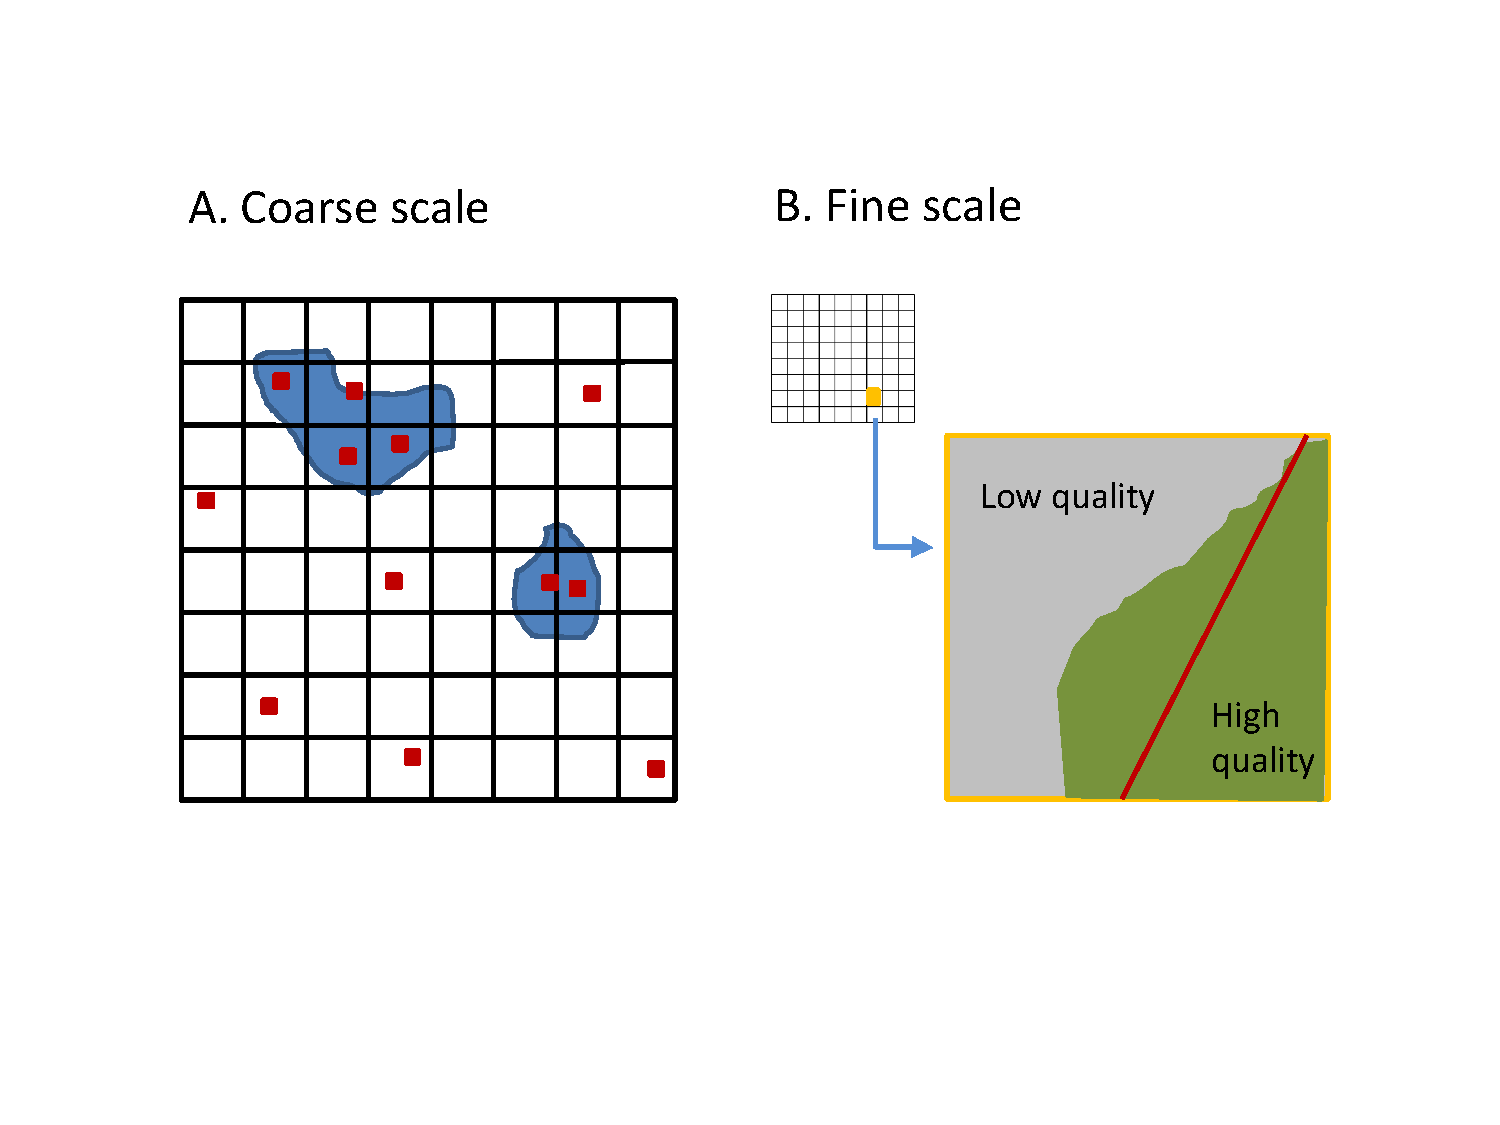
\includegraphics[width=170mm]{Pref_sampling_diag.pdf}
\caption{A depiction of two types of preferential sampling.  In (A), an investigator preferentially places point transects (red squares) within regions of high known animal density (blue polygons).  This can cause bias in abundance or occupancy estimators unless this a priori knowledge about density is explicitly modeled.  In (B), a fine scale version of preferential sampling occurs when a line transect (red line) is intentionally placed across a region of high quality habitat.  If a landscape is discretized into homogeneous survey units (as in a grid), it is essential that the habitat surveyed within each survey unit be randomly determined when estimating abundance.  If not, bias (usually positive) can be expected.}
\label{fig:pref}
\end{center}
\end{figure*}

\begin{figure*} %[ht]
\begin{center}
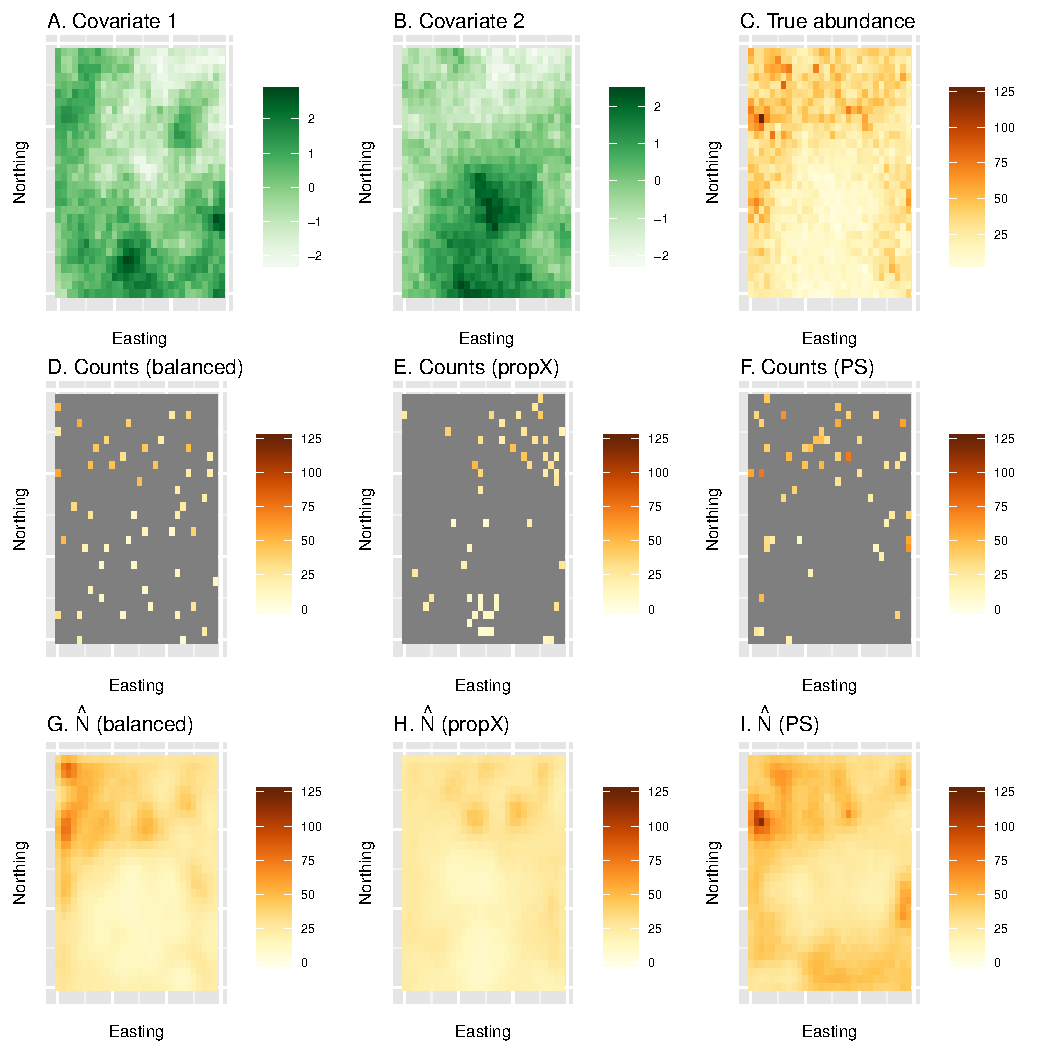
\includegraphics[width=170mm]{PS_maps.pdf}
\caption{An example of a single simulation replicate examining the effect of preferential sampling on estimates of abundance from a species distribution model.  First, two spatially autocorrelated covariates are generated (panels A-B).  Second, true abundance is generated conditional on these covariates (C).  Next, three hypothetical sampling designs are employed to generate animal counts, including a spatially balanced sample (D), a design where sampling is proportional to values of a modeled covariate (E), and where sampling is preferential - i.e. more likely to occur where abundance is high (F).  Finally, spatially explicit estimates of abundance are generated using a traditional SDM to each of the count datasets (G-I).  Although the map produced in (I) does not look particularly bad in this instance, preferential sampling led to estimates of abundance that were biased 20\% high.}
\label{fig:PS_sims}
\end{center}
\end{figure*}



\end{document}

%http://www.plosone.org/article/info:doi/10.1371/journal.pone.0036527
